\documentclass[10pt]{article}
\usepackage[utf8]{inputenc}
\usepackage[includehead, headheight=10mm, margin=15mm ]{geometry}
\usepackage{amsmath}
\usepackage{amsthm}
\usepackage{amsfonts}
\usepackage{xcolor}
\usepackage{graphicx}
\usepackage{titling}
\usepackage{fancyhdr}
\usepackage{listings}

\title{APPM 4600 Homework 5}
\author{Edward Wawrzynek}
\date{4 October 2024}

\newcommand*{\dif}{\mathop{}\!\mathrm{d}}
\renewcommand{\vec}{\mathbf}

\makeatletter
\def\@maketitle{%
  \newpage
  \null
  \vskip 1em%
  \begin{center}%
  \let \footnote \thanks
    {\LARGE \@title \par}%
    \vskip 1em%
    {\normalfont \@date}
  \end{center}%
  \par
  \vskip 1em}
\makeatother

\begin{document}

\pagestyle{fancy}
    \fancyhf{} % clear all header and footer fields
    \fancyhead[L]{\thetitle}
    \fancyhead[R]{\theauthor}

\makeatletter
\begin{center}
    {\Large \@title}
    \vskip 1mm
    {\normalfont \@date}
    \vskip 1em
\end{center}
\makeatother

\begin{enumerate}
    \item \begin{enumerate}
      The code used in this question is listed at the end of the question.
      \item Iteration over the system converges to the approximate root \begin{align*}
          \begin{bmatrix}
            x \\
            y
          \end{bmatrix} \approx \begin{bmatrix}
            0.5 \\
            0.8660254037844386
          \end{bmatrix}.
      \end{align*} This convergence is numerically of first order (\(\alpha \approx 0.98811\)), although it converges to the desired tolerance in fewer iterations than lazy Newton.

      \item The system has Jacobian \begin{align*}
          J(x,y) = \begin{bmatrix}
            6x & -2y \\ 3y^2 - 3x^2 & 6xy
          \end{bmatrix}.
      \end{align*} At \(x=y=1\), this is \begin{align*}
          J(1,1) = \begin{bmatrix}
            6 & -2 \\ 0 & 6
          \end{bmatrix},
      \end{align*} with inverse \begin{align*}
          J(1,1)^{-1} = \begin{bmatrix}
            \frac{1}{6} & \frac{1}{18} \\ 0 & \frac{1}{6}
          \end{bmatrix}.
      \end{align*} Thus, the choice of the matrix implements lazy newton's method, where the Jacobian is only evaluated at the initial guess and never updated in the iteration.

      \item Newton's method converges to the approximate root \begin{align*}
        \begin{bmatrix}
          x \\
          y
        \end{bmatrix} \approx \begin{bmatrix}
          0.5 \\
          0.8660254037844387
        \end{bmatrix},
      \end{align*} which is similar to the previous iteration. This convergence is of first order (numerically, \(\alpha \approx 1.0078\)).

      \item The exact solution is simply \begin{align*}
        \begin{bmatrix}
          x \\
          y
        \end{bmatrix} \approx \begin{bmatrix}
          \frac{1}{2} \\
          \frac{\sqrt{3}}{2}.
        \end{bmatrix}
      \end{align*}

      {\small \lstinputlisting[language=Python]{hw5_1.py}}
    \end{enumerate}

    \newpage
    \item We have iterative step \begin{align}\label{eq:iter}
        \begin{split}
        x_{n+1} = f(x_n, y_n) &= \frac{1}{\sqrt{2}}\sqrt{1+(x_n+y_n)^2} - \frac{2}{3}, \\
        y_{n+1} = g(x_n, y_n) &= \frac{1}{\sqrt{2}}\sqrt{1+(x_n-y_n)^2} - \frac{2}{3}.
        \end{split}
    \end{align}
    
    We are looking for some closed rectangular region where the partial derivatives of \(f\) and \(g\) are continuous and \begin{align}\label{eq:bound}
        |f_x| \leq \frac{1}{2},\;|f_y| \leq \frac{1}{2},\;|g_x| \leq \frac{1}{2},\;\mathrm{and}\;|g_y| \leq \frac{1}{2}.
    \end{align}

    The component functions \(f\) and \(g\) have partials \begin{align*}
        f_x(x,y) = f_y(x,y) &= \frac{x+y}{\sqrt{2}\sqrt{(x+y)^2+1}}, \\
        g_x(x, y) = -g_y(x,y) &= \frac{x-y}{\sqrt{2}\sqrt{(x-y)^2+1}},
    \end{align*} which are continuous everywhere in \(\mathbb{R}^2\).

    The largest region over which \eqref{eq:bound} is satisfied is \(D = [-\frac{1}{2}, \frac{1}{2}] \times [-\frac{1}{2}, \frac{1}{2}]\). By theorem 10.6, any fixed point iteration of \eqref{eq:iter} with initial guess \((x_0, y_0) \in D\) will converge to some fixed point \(\mathbf{p} \in D\).

    \newpage

    \item \begin{enumerate}
      \item We start at some initial guess \(\vec{x_0} = (x_0, y_0)\), where \(f(\vec{x_0}) \neq 0\). We wish to find \(f(\vec{x}) = 0\), so we want to move in the direction of the gradient of \(f\), which is the line given by \begin{equation}\label{eq:normal_line}
        \vec{x}-\vec{x_0} = \alpha \nabla f(\vec{x_0}),
      \end{equation} where \(\alpha \in \mathbb{R}\).
      About the guess \(f\) has first order Taylor expansion \begin{align}\label{eq:taylor}
        \begin{split}
          f(\vec{x}) &\approx f(\vec{x_0}) + (\vec{x}-\vec{x_0})\cdot \nabla f(\vec{x_0}).
        \end{split}
      \end{align} Substituting \eqref{eq:normal_line} into \eqref{eq:taylor}, we have \begin{align*}
          f(\vec{x}) &\approx f(\vec{x_0}) + \alpha \nabla f(\vec{x_0}) \cdot  \nabla f(\vec{x_0}) \\
          &= f(\vec{x_0}) + \alpha \nabla^2 f(\vec{x_0}).
      \end{align*} We want \(f(\vec{x}) = 0\), so we have \begin{align*}
          \alpha = -\frac{f(\vec{x_0})}{\nabla^2 f(\vec{x_0})}.
      \end{align*} Substituting this back into \eqref{eq:taylor}, we have \begin{align*}
          \vec{x} = \vec{x_0} - \frac{f(\vec{x_0})}{\nabla^2 f(\vec{x_0})}\nabla f(\vec{x_0}),
      \end{align*} which gives the iterative step \begin{align*}
          \begin{pmatrix}
            x_{n+1} \\ y_{n+1}
          \end{pmatrix} = \begin{pmatrix}
            x_n - \frac{f(x_n, y_n) f_x(x_n, y_n)}{f_x(x_n, y_n)^2 + f_y(x_n, y_n)^2} \\
            x_y - \frac{f(x_n, y_n) f_y(x_n, y_n)}{f_x(x_n, y_n)^2 + f_y(x_n, y_n)^2}
          \end{pmatrix},
      \end{align*} as expected.
    \end{enumerate}

    \item The code used to answer this question is listed at the end of the question.
    
    We start the iteration at \((1,1,1)\) and converge to the point \begin{align*}
        \vec{x^*} \approx \begin{pmatrix}
          1.09364232 \\ 1.36032838 \\ 1.36032838
        \end{pmatrix}.
    \end{align*} This convergence is indeed second order (numerically, \(\alpha \approx 2.013\)). This can be seen in the plot of \(\ln || \mathbf{x_{n+1}} - \mathbf{x^*} ||\) vs \(\ln || \mathbf{x_{n}} - \mathbf{x^*} ||\) below, where \(|| \cdot  ||\) is the \(L^2\) norm.

    \begin{center}
      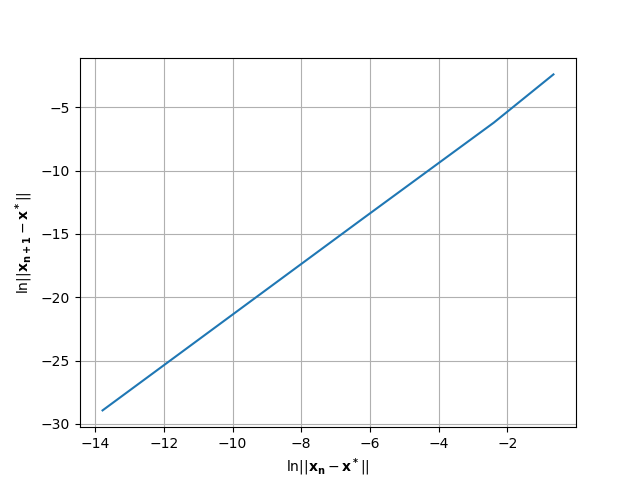
\includegraphics[width=0.5\textwidth]{hw5_3b.png}
    \end{center}

    {\small \lstinputlisting[language=Python]{hw5_3b.py}}
\end{enumerate}


\end{document}